\documentclass[11pt]{article} % do not change this line
\input{BigDataStyle.txt}      % do not change this line
\usepackage[hidelinks]{hyperref}
\usepackage[export]{adjustbox}
\usepackage{amsmath,amsfonts,amssymb,amsthm,latexsym,graphicx,url,bookmark}

\emergencystretch=5mm
\tolerance=400
\allowdisplaybreaks[4]

\theoremstyle{plain}
\newtheorem{theorem}{Theorem}[section]
\newtheorem{proposition}[theorem]{Proposition}
\newtheorem{corollary}[theorem]{Corollary}
\newtheorem{lemma}[theorem]{Lemma}
\newtheorem{problem}[theorem]{Problem}

\theoremstyle{definition}
\newtheorem*{remark}{Remark}

\title{Machine Learning for Investing Behaviours on Cryptocurrencies}
\author{Chengkai Lu}

\newcommand{\Programme}{Data Science and Analytics with a Year in Industry}

\begin{document}
\maketitle

\declaration

\begin{abstract}
  Your abstract goes here.
\end{abstract}

\section{Introduction}
\subsection{Motivation}
\subsection{Aims And Objectives}
\subsection{Project Structure}
\subsubsection{Technologies}
\subsubsection{Programme Structure}
\subsubsection{Report Structure}

\section{Background Research}
\subsection{Correlation Analysis}
\subsection{Dimensionality Reduction}

It is always challenging to analyse a dataset with high-dimensional data points. Due to the curse of dimensionality, which was discovered by Richard Ernest Bellman in 1961, higher dimensional space increases the difficulties of analysing and organising data exponentially\cite{wiki/cod:2018}. Especially in machine learning, given a certain number of samples, the accuracy of predictions on these samples will increase followed by the rising dimensions to a peak but then gradually drop. This is known as Hughes phenomenon\cite{hughes/itoit:1968}.

\begin{figure}[htp]
  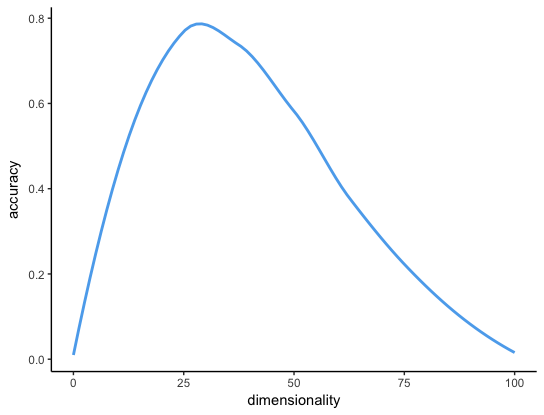
\includegraphics[width=0.8\linewidth, center]{resources/dimensionality.png}
  \caption{Hughes phenomenon}
  \label{fig:hughes}
\end{figure}

In order to reduce the dimensionality, there are two approaches can be implemented:
\begin{itemize}
  \item Feature Selection: 
  \item Feature Extraction:
\end{itemize}

The reasons and benefits of executing dimensionality reduction can be summarised as follow:
\begin{enumerate}
  \item Computational efficiency
  \item Statistical generalisation
  \item Better explanation
\end{enumerate}

\subsubsection{Principal Component Analysis}
\subsection{Clustering}

Clustering, cluster analysis or data segmentation is a non-parametric algorithm in the subtree of unsupervised learning. It is used to separate data into different groups using their natural dissimilarities. Unlike supervised learning, this type of learning algorithms does not have any indicator for assessing the quality of results, and this means that it does not have any meaning or objective itself. Instead, it discovers the distribution of data and uses the definition given by people who have the specific domain knowledge. By giving the rules for partitioning data self-defined meanings, useful information can be obtained and utilised in different domains\cite{hastie/etal:2009}.

Generally, 

\subsubsection{K-means Clustering}

An example of a reference:
\cite{adam/dpapa:2017}.

\subsection{Recurrent Neural Network}
\subsubsection{Long Short-Term Memory}

\section{K-means Clustering on Price Fluctuations}
\subsection{Data Prepocessing}
\subsubsection{Data Formats}
\subsubsection{Normalisation}
\subsection{Data Analysis}
\subsubsection{Shifting Along Timeline}
\subsubsection{Model Training}
\subsection{Result}

\clearpage

\section{LSTM on Highest/Lowest Nextday Growth Prediction}
\subsection{Data Prepocessing}
\subsubsection{Data Formats}
\subsubsection{Normalisation}
\subsubsection{Training Set and Validation Set}
\subsection{Data Analysis}
\subsubsection{Activation Functions}
\subsubsection{Parameters}
\subsubsection{Regularisation}
\subsubsection{Loss Function}
\subsubsection{Model Training}
\subsection{Result}
\subsubsection{Back Test}

\section{Performance}
\subsection{K-means Clustering}
\subsection{Long Short-Term Memory}

\section{Conclusion and Evaluation}
\subsection{Visualisation}
\subsection{Further Work}

\section{Appendix}
\subsection{Programme Usage}

\bibliographystyle{plain}
\bibliography{bibliography}
\end{document}
